\documentclass[tikz,border=5pt]{standalone}

\usepackage{pgfplots}
\pgfplotsset{compat=1.18}

\begin{document}
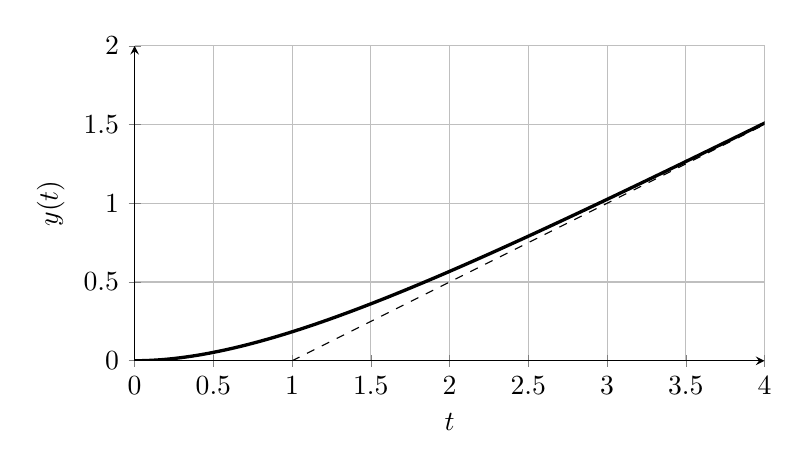
\begin{tikzpicture}
    \begin{axis}[
        width=8cm,
        height=4cm,
        xmin=0, xmax=4,
        ymin=0, ymax=2,
        scale only axis,
        axis lines=left,
        xlabel={$t$},
        ylabel={$y(t)$},
        grid=both,
        unbounded coords=discard,
        restrict y to domain=0:2,
        axis equal image,
    ]
    \addplot[domain=0:7, samples=200, very thick]
        {max(0, 0.5*(x-1) + 0.5*exp(-x))};
    \addplot[domain=1:4, samples=2, dashed]
        {0.5*(x-1)};
    \end{axis}
\end{tikzpicture}
\end{document}
